% !TeX root = Trafficsimulation_Documentation.tex

\chapter{Design}
\label{Design}

In diesem Kapitel werden die Implementierungen der einzelnen Komponenten sowie deren Schnittstellen zu anderen Komponenten dokumentiert.

\thispagestyle{standard}
\pagestyle{standard}

\section{Strassensystem}
\label{Strassensystem}

\subsection{Ampeln}

\subsection{Strassen}

\subsection{Kreuzungen}

\section{Fahrzeuglogik}
\label{Fahrzeuglogik}

\section{Ampelsteuerung}

\section{Hindernisse}
\label{Hindernisse}

Mit einem Klick der Maus sollen überall in der Welt Hindernisse platziert werden, welche anschließend von Fahrzeugen umfahren werden müssen. Durch einen weiteren Klick auf ein Hindernis soll dieses wieder gelöscht werden. 

Unity ermöglicht das Erstellen von GameObjects zur Laufzeit. Durch den Klick auf die Welt können die Koordinaten des Klicks festgestellt werden und somit das GameObject, welches bereits beim Start der Verkehrssimulation geladen wurde, platziert werden.

Durch das Halten eines Buttons auf der Tastatur soll die Erstellung von Hindernissen aktiviert werden. Dies verhindert, dass der Benutzer unbeabsichtigt zu viele Hindernisse erstellt.

\section{Aus- und Einfahren von Fahrzeugen anderer Gruppen}

Mit dem Plugin `Unity3D.Amqp` (\url{https://github.com/CymaticLabs/Unity3D.Amqp}) für Unity ist es möglich einen RabbitMQ-Server direkt in Unity einzubinden.

Die Konfiguration der Serverdaten werden dabei direkt in den Menüeinstellungen von Unity vorgenommen. Die verwendete Konfiguration ist in Abbildung \ref{img:rabbit} zu sehen.

\begin{figure}[H]
\begin{center}
	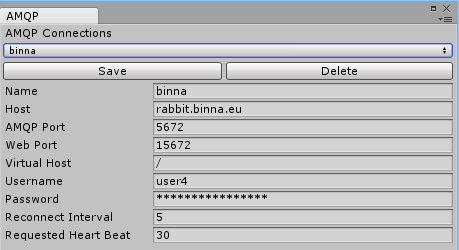
\includegraphics[width=0.9\textwidth]{BilderAllgemein/rabbitconfig.png}
\end{center}

	\caption{Einstellungen RabbitMQ}

	\label{img:rabbit}
\end{figure}

Jede Gruppe bekam einen eigenen Benutzer samt Passwort. Damit man Nachrichten empfangen kann, muss man sich auf eine `Queue` subscriben.

Das Plugin stellt anschließend Methoden zur Verfügung. Eine solche Methode ist \texttt{OnMessageReceived()}. Damit lässt sich eine eingehende Nachricht an ein Objekt in der Spielwelt weitergeben. Das Objekt kann daraufhin reagieren, beispielsweise ein Auto erzeugen.

\begin{figure}[H]
\begin{center}
	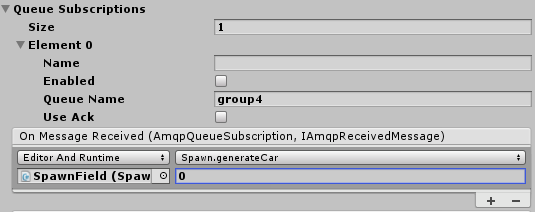
\includegraphics[width=0.9\textwidth]{BilderAllgemein/rabbitqueue.png}
\end{center}

	\caption{RabbitMQ Queue}

	\label{img:rabbitq}
\end{figure}

In Abbildung \ref{img:rabbitq} sieht man wie eine eingehende Nachricht beim Objekt \texttt{SpawnField} eine Methode aufruft.